\begin{mdframed}[style=warning]
	\textbf{Conceptos}
		\begin{enumerate}
			\item El período de revolución de Júpiter alrededor del sol es $12$ veces el período de la Tierra. Asumiendo que las órbitas planetarias son circulares encuentre:
			\begin{enumerate}[a)]
				\item Cuántas veces la distancia entre Júpiter y el Sol es mayor que la distancia entre el Sol y la Tierra?
				\item La velocidad y aceleración de Júpiter en el marco de referencia heliocéntrico.
			\end{enumerate}
			\item A mayor altura, ¿la energía cinética para poner un satélite en órbita o la energía para mantenerse en órbita es mayor?
		\end{enumerate}
\end{mdframed}






\begin{mdframed}[style=warning]
	\begin{ejercicio}
		Tres Cuerpos idénticos de masa $m$ están situados en los vértices de un triángulo equilátero de lado $L$. Cada uno de los cuerpos se puede mover en una órbita circular circunscrita al triángulo original. Si las únicas fuerzas que actúan sobre los cuerpos son las atracciones gravitacionales mutuas, ¿cuál será la rapidez de su movimiento?
	\end{ejercicio}
\end{mdframed}






\begin{mdframed}[style=warning]
	\begin{ejercicio}
		Dos estrellas de masa $M$ y $m$, separadas una distancia $d$, dan vueltas en órbitas circulares en torno a su centro de masa. Demuestre que cada estrella tiene un periodo dado por
			$$ T^2 = \frac{4\pi ^2 d^3}{G (M + m)}. $$
	\end{ejercicio}
\end{mdframed}









\begin{mdframed}[style=warning]
	\begin{ejercicio}
		Encuentre una expresión que modele el valor de $g$ dentro de la tierra, asumiendo que es una esfera uniforme.
	\end{ejercicio}
\end{mdframed}



















\begin{mdframed}[style=warning]
	\begin{ejercicio}
		Se tiene un sistema esférico con un hueco que toca el centro y el borde de la esfera. El radio de la esfera es $R = 4cm$ y su masa antes del hueco era $M_o = 2.95kg$. ¿Con qué fuerza gravitatoria, la esfera de plomo ahuecada, atrae a una pequeña esfera de masa $m = 0.431kg$ que se encuentra a una distancia $d = 9cm$ del centro de la esfera de plomo, en la línea recta que une los centros de las esferas y del hueco?
		\begin{figure}[H]
			\centering
			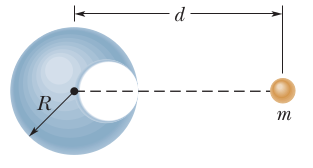
\includegraphics[scale=0.5]{./img/p4.png}
			\caption{Figura problema 4.}
			\label{p4}
		\end{figure}
	\end{ejercicio}
\end{mdframed}















%%%